\section{Methodology}
We use a modified version of Apriori algorithm combined with frequency position tables in order to calculate single byte-length tokens and frequently occurring substrings using choice operators and position constraints \cite{WANG2012992}. RExACtor also uses genetic sequence alignment to find commonalities in payloads and encodes this alignment in order to create a regular expression from it. Our system performs better than previous work in memory space allocation by additionally using position frequencies to specify character classes and length constraints instead of generic wildcards. This creates real-time performance optimization in the scanner. Furthermore, unlike previous solutions our system requires no packet buffering or traffic flow information to do its identification.

RExACtor is made up of component modules which perform various stages of data processing and analysis in order to create optimal regular expressions. The flow of the system is shown in Figure~\ref{f:diagram}. RExACtor takes in as input packet capture (PCAP) files and extracts session payload strings for supported protocols. The input can be of any mix of traffic types, and is therefore well-suited to learning in the wild from real network captures. This extraction layer takes in parameters from the command line interface to select a supported protocol and message type to specifically isolate training data from the mixed input. It also offers an extraction option for the full data layer for analysis. For our experiments, we selected HTTP, SIP, and RTSP as protocols and extracted request and response session payloads for each of them.

\begin{figure}[hbt!]
  \begin{center}
    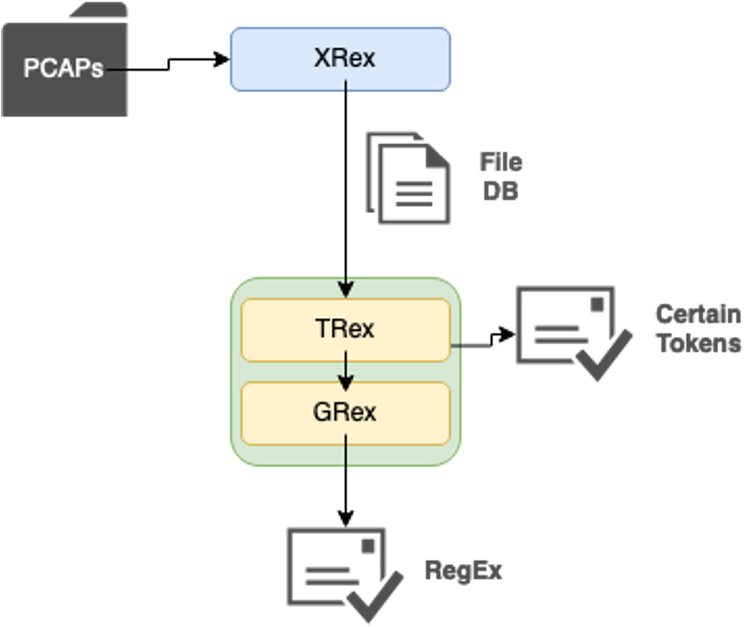
\includegraphics[width=0.6\columnwidth]{chapters/3/img/diagram.png}
    \caption{High-level diagram of signature construction in RExACtor. The system produces certain tokens and regular expressions which can be used with the HRex Scanner or any external filtering/sniffing application.}
    \label{f:diagram}
  \end{center}
\end{figure}

\subsection{TRex: Apriori Tokenization of Packet Payloads}
Inside the starting lines, some substrings appear frequently across packets and thus can be used as string literals in signatures. In the SIP protocol, the line ``SIP/2.0" appears at the end of all starting lines in all our training data SIP requests. In HTTP, the protocol name and version ``HTTP/1.1" appear consistently, as well. We use a modified version of the Apriori Algorithm \cite{Toivonen2017} in order to find frequently occurring substrings, or \textit{tokens}, in our packet strings. Shim et al also use Apriori in SigBox for content strings \cite{Shim2017SigBoxAS}.

Apriori is an algorithm used for finding frequent item sets and association rules from databases. The algorithm uses a bottom-up approach to combine items into incrementally larger item sets, keeping only those sets which meet some minimum threshold of support. The support of an itemset in the database is defined as the number of instances of the itemset in the transactions over the total number of transactions \cite{Toivonen2017}.

\vspace{\baselineskip}

\[\text{Support(X)} = \frac{\text{Instances of X in transactions}}{\text{Number of transactions}}\] \par

\vspace{\baselineskip}

In the formal definition provided by Rakesh Agrawal \cite{Agrawal}, let $I = \{i_{1},i_{2},i_{3}...i_{n}\}$ be a set of items of length \textit{n} and $D = \{t_{1},t_{2},t_{3}...t_{n}\}$ be the set of transactions known as a database. Every transaction $t_{i}$ has a unique identifier in $D$ and $\forall t_{i} : x \in t_{i} \rightarrow x \in I$, or every transaction is a subset of items in $I$. Apriori relies on the anti-monotonicity of the support of itemsets which assumes that all subsets of a frequent itemset must also be frequent, and all supersets of an infrequent itemset must also be infrequent. \par

\begin{algorithm}
\SetAlgoLined
\KwResult{Frequent Itemsets}
 $k=1$, $I_{k} = \{\text{frequent item sets of size 1}\}$\;
 \While{\text{(}$I_{k} \neq \emptyset$\text{)}} {
 $C_{k+1} = apriori\_gen(I_{k})$\;
 \For{$t \in D$} {
      $C_{t} = subset\text{(}C_{k+1}, t\text{)}$\;
      \For{$c \in C_{t}$} {
      c.count++\;
      }
      $I_{k+1} = c \in C_{k+1} \text{ }\vert \text{ } c.count \geq minsup$\;
   }
   $k = k + 1$\;
  }
  $\text{tokens} = \cup_{k}I_{k}$\;
  \Return $\text{prune\_substrings(tokens)}$\;
 \caption{Modified Apriori Algorithm \cite{Agrawal}}
\end{algorithm}

We mine tokens using a modified Apriori approach. Each packet string derived from pre-processing is treated as an individual line in the database. TRex uses a sliding window algorithm of length $k$ to create substring items which are grouped into a list treated as a single transaction. We initialize the window size to $k=2$ in order to prevent likely frequent but meaningless single-byte tokens and set the maximum itemset length $l=1$. The first iteration calculates the frequency of substrings of length $k=2$ and each subsequent loop increments $k$ until no more frequent itemsets (substrings) are found.

Because the order of substrings matters in regular expression matching, we limit the maximum itemset length to 1. We increase item size instead by increasing the window size, thereby preserving order of characters in the modified algorithm. At each iteration, we also prune the resulting token set by replacing tokens $i$ in the current set $S = \{I_{k_{0}}, I_{k_{1}}, I_{k_{2}}...I_{k_{n}}\}$ with any strings $j$ in the result set $I_{k_{n+1}}$ which are superstrings of $i$ and $ support\text{(i)} = support\text{(j)}$. This reduces redundancy of tokens such as ``SIP" and ``SIP/" when the sets are unioned together.

\begin{figure}[hbt!]
  \begin{center}
    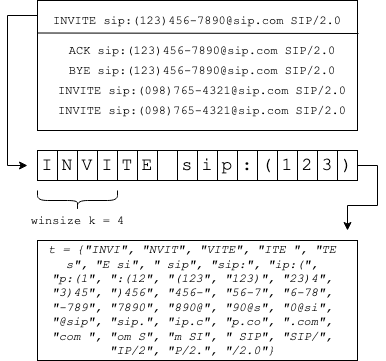
\includegraphics[width=0.7\columnwidth]{chapters/3/img/slidingwindow.png}
    \caption{Modified Apriori Algorithm for string packet data using a sliding window algorithm. The sliding window process is repeated for all packet strings in the database file to make the full set of transactions.}
    \label{f:slidingwindow}
  \end{center}
\end{figure}

\textit{Certain tokens}. Substrings with support equal to 1.0. \par
\textit{Frequent tokens}. Substrings with support equal to a manually configured threshold. For example, in SIP 2.0 the method words \texttt{INVITE}, \texttt{ACK}, and \texttt{BYE} frequently occur in request packets. \par

In order to give positional context to tokens, we introduce position frequency tables from natural language processing (NLP). This allows TRex to compute prefix and suffix groups from frequent tokens. Given a list of tokens $t_{1}, t_{2}, t_{3},...t_{n}$, TRex constructs a position frequency table for each token in each starting line in the database. The resulting vector $V=[\{ t_{1}:pos_{1}, t_{2}:pos_{2}, t_{3}:pos_{3},...t_{n}:pos_{n}\}, \{ t_{1}:pos_{1}, t_{2}:pos_{2}, t_{3}:pos_{3},...t_{n}:pos_{n}\}...]$ is referenced for tokens which occur at $pos=0$. If the sum of support for those tokens found at $pos=0$ is approximately 1.0 with respect to a minimal noise threshold, all tokens in this subset are captured in a prefix group. In the SIP request example, the methods \texttt{INVITE}, \texttt{ACK}, and \texttt{BYE} would be captured and separated with regular expression choice operators and a beginning position constraint in the following manner: $\string^\text{(\texttt{INVITE}}\vert\text{\texttt{ACK}}\vert\text{\texttt{BYE}}\text{)}$. \par

For suffixes, TRex uses string manipulation to reverse both the tokens and starting lines, which intuitively reverses the position significance also so that $pos=len(starting\_line)$ is now decides what goes into the capture group. Frequent tokens are reversed back to their original order before being inserted into the suffix, and choice operators and an end position constraint are appended. Example suffixes may include response codes, status codes or messages, or version numbers of protocols. An example output from TRex configured for HTTP requests and run on data containing both v. 1.0 and v. 1.1 requests may derive a suffix such as $\text{(\texttt{HTTP/1.0}}\vert\text{\texttt{HTTP/1.1}}\text{)\$}$.

In addition to forming prefixes and suffixes, position frequency tables also give meaning to single-byte tokens which occur with $freq=1.0$ at a fixed position. Wang et al found that some protocols have distinctive features at fixed offsets. As an example, they showed that the QQ messaging application always ends its packets with the byte \texttt{0x03}, indicating the end of a message \cite{WANG2012992}. We calculate position frequency tables similar to their approach for each character in each starting line and repeat the process in reverse in order to find single-byte tokens. These tokens are then added to the certain tokens set for future regular expression insertion. The substring tokens are then extracted from the relevant database lines and the remainder is preserved for the alignment stage.

\subsection{GRex: Genetic Sequence Alignment of Common Substrings}

GRex uses principles from genetic sequencing algorithms in order to pairwise align the remaining starting line data. Because we pre-process data into starting lines and TRex removes the found prefixes and suffixes to concentrate on only data which should be aligned, it is appropriate in our system to use a global alignment algorithm which attempts to align the entire sequence pair. We also use progressive alignment to sequentially align pairwise sequences to derive a resulting optimal alignment.

We chose to utilize the Needleman-Wunsch Algorithm for scoring and global alignment \cite{NEEDLEMAN1970443}. As a dynamic programming algorithm, Needleman-Wunsch utilizes a 2D scoring matrix which rewards matching characters and penalizes mismatches according to predefined parameters. Furthermore, a gap penalty is introduced to account for insertions/deletions (indels) in the string alignment. The principle of the algorithm is to greedily maximize the score of alignment per cell. Each cell in the matrix also contains a pointer value which points to the origin of the highest score and will aid in the final trace-back stage \cite{blast}. The score function $F$ with gap score $g$, sequence $A = \{a_{1}, a_{2}, a_{3},...a_{n}\}$, and sequence $B = \{b_{1}, b_{2}, b_{3},...b_{k}\}$ is defined as follows:\par

\begin{equation}
  F(i,j) = max
    \begin{cases}
    F(i-1, j-1) + score(a_{i}, b_{j}) \\
    F(i-1, j) + g \\
    F(i, j-1) + g \\
    \end{cases}
\end{equation}
\vspace{\baselineskip}

In the initialization phase, the first row and column are set as the gap score times the distance from the origin, which is the upper left most corner of the matrix. From here, the algorithm recursively computes the match score, horizontal gap score, and vertical gap score for each cell in the matrix. The match score is calculated from the preceding diagonal cell's score and the score of alignment of the two characters (match or mismatch). The horizontal gap score is the sum of the score to the left and the and the gap score. Similarly, the vertical gap score is the sum of the cell above and the gap score. The cell is set to the maximum of these values and the pointer to the cell (left, vertical, or diagonal) where the maximum came from. Once the matrix has been filled, the pointers are used to trace back through to find the highest-scoring alignment \cite{blast}. Figure \ref{f:needlemanwunsch} demonstrates this scoring algorithm in a matrix.

\begin{figure}[hbt!]
  \begin{center}
    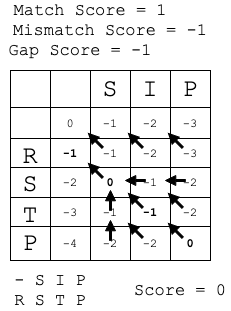
\includegraphics[width=0.3\columnwidth]{chapters/3/img/needlemanwunsch.png}
    \caption{Scoring matrix example of the Needleman-Wunsch Algorithm. Traceback follows from the right bottom corner to the top left cell. The alignment results in the maximum possible score = 0.}
    \label{f:needlemanwunsch}
  \end{center}
\end{figure}

GRex modifies the Needleman-Wunsch algorithm to encode Greek symbols into our alignments which represent specific character classes, insertions and deletions, and mismatches which will later be decoded in the final translation step and used to generate regular expressions. Table \ref{table:greekencoding} provides a key to GRex's Greek symbol encoding. Previous work used an encoding algorithm for indels and mismatches \cite{WANG2012992}, but we created our own encoding schema for GRex and expanded this to also incorporate defining character classes. Specifically, we encode symbols based on whether a character in a given position is or is not a white space character, alphabet character, or digit. Table \ref{table:regexes} shows the regular expression operators GRex derives from these encodings at the translation step.

\begin{table}
\begin{center}
\begin{tabular}{|c | l|}
  \hline
  $\Phi$ & insertion/deletion \\
  \hline
  $\Delta$ & mismatch \\
  \hline
  $\psi$ & gap \\
  \hline
  $\Sigma$ & alphabet character \\
  \hline
  $\omega$ & not alphabet character\\
  \hline
  $\Pi$ & digit \\
  \hline
  $\lambda$ & not digit \\
  \hline
  $\Omega$ & white space character \\
  \hline
  $\sigma$ & not white space character \\
  \hline
\end{tabular}
\caption{Greek Symbols For GRex Encoding}
\label{table:greekencoding}
\end{center}
\end{table}

\begin{table}
\begin{center}
\begin{tabular}{|c|c|p{0.5\linewidth}|}
  \hline
  Type & Symbol & Definition \\
  \hline
  & $.$ & matches any character \\
  \cline{2-3}
  & [] & matches any character in brackets \\
  \cline{2-3}
  & [$\string^$] & matches any character not in brackets \\
  \cline{2-3}
  & \textbackslash s & white space character \\
  \cline{2-3}
  character class & \textbackslash d & digit \\
  \cline{2-3}
  & \textbackslash w & word character \\
  \cline{2-3}
  & \textbackslash S & not white space character \\
  \cline{2-3}
  & \textbackslash D & not digit \\
  \cline{2-3}
  & \textbackslash W & not word character \\
  \hline
  & * & matches zero or more times \\
  \cline{2-3}
  & ? & matches at most one time \\
  \cline{2-3}
  quantifier & + & matches one or more times \\ \cline{2-3}
  & \{$m,n$\} & matches between $m$ and $n$ times \\
  \cline{2-3}
  & \{$m$,\} & matches $m$ or more times \\
  \cline{2-3}
  & \{,$n$\} & matches at most $n$ times \\
  \hline
  & $\string^$ & matches beginning of data \\
  \cline{2-3}
  other & \$ & matches end of data \\
  \cline{2-3}
  & () & capture group \\
  \cline{2-3}
  & $\vert$ & OR operator \\
  \hline
\end{tabular}
\caption{Supported Regular Expression Operators}
\label{table:regexes}
\end{center}
\end{table}

The encoding process runs in a progressive manner, such that two strings are aligned, compared, and encoded, and that return is then passed again and compared against another string in the sequence. Once aligned using the Needleman-Wunsch algorithm, the character types of each index are compared. Depending on the type of character, the returned string from this process is appended with a representation of either the character itself if the indexes are matching or a Greek character encoding otherwise. Once the new string is fully appended, it is returned to the loop. This returned string is compared to the next entry within the data. This process loops until every line from the packet data is aligned into the final encoding.

In order to create the regular expression, the replacement function is run against the generated string. Each index is checked and replaced with the regular expression counterpart with correct special character escaping. The final regular expression is constructed from the symbolic string. Frequent tokens are combined with choice operators and positional constraints $\string^$ and $\$$ for prefixes and suffixes, respectively. Prefixes are appended to the beginning of the generated regular expression, and suffixes to the end.

\subsection{HRex: High Performance Regular Expression Scanning}
The final component is a sniffing application written in C++ which reads in PCAP files using \texttt{libpcap} and performs regular expression scanning with Intel's Hyperscan library~\cite{hyperscan}. Hyperscan provides significant performance improvement over other commercial but popular tools like Snort due to its reduction of duplicate operations in string and pattern matching and use of single-instruction, multiple data (SIMD) operations. In their experimentation, creators of Hyperscan found it outperformed Snort by a factor of 8.7~\cite{hyperscanusinex}. Our string literal tokens created by RExACtor's TRex can be applied in a pre-filter system like Snort, as well. Furthermore, Hyperscan does additionally support string literal, or keyword, matching. We provide both solutions for flexibility in real-world applications as the network capture environment is rarely one-size-fits-all. As our tokens are learned via unsupervised learning, they do not require manual analysis and thus scale well to larger, unknown data sets.
